\chapter{Конструкторская часть}

\section{Схемы алгоритмов}

Для алгоритма Винограда худшим случаем являются матрицы с нечётным общим размером, а лучшим -- с чётным, из-за того что отпадает необходимость в последнем цикле.

Данный алгоритм можно оптимизировать.
\begin{itemize}
	\item Замена  выражения $x = x + k$ на $x += k$;
	\item Замена вызова функции вычисления длины строки на заранее вычисленное значение.
	\item Замена деления на 2 на побитовый сдвиг.
\end{itemize}

На рисунке 2.1 приведена схема стандартного алгоритма умножения матриц.

На рисунках 2.2 и 2.3 представлена схема алгоритма Винограда и схема оптимизированного алгоритма Винограда. 

\begin{figure}[ht!]
	\centering
	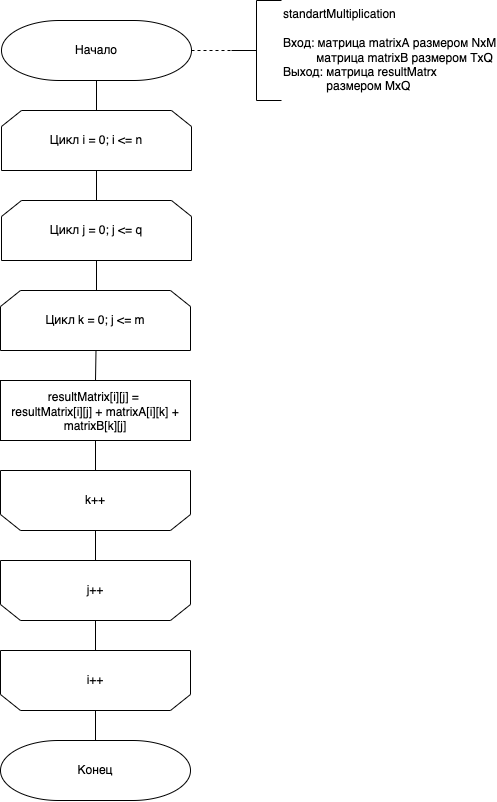
\includegraphics[width=0.9\linewidth]{img/Standard.png}
	\caption{Схема стандартного алгоритма умножения матриц}
	\label{fig:mpr}
\end{figure}

\begin{figure}[ht!]
	\centering
	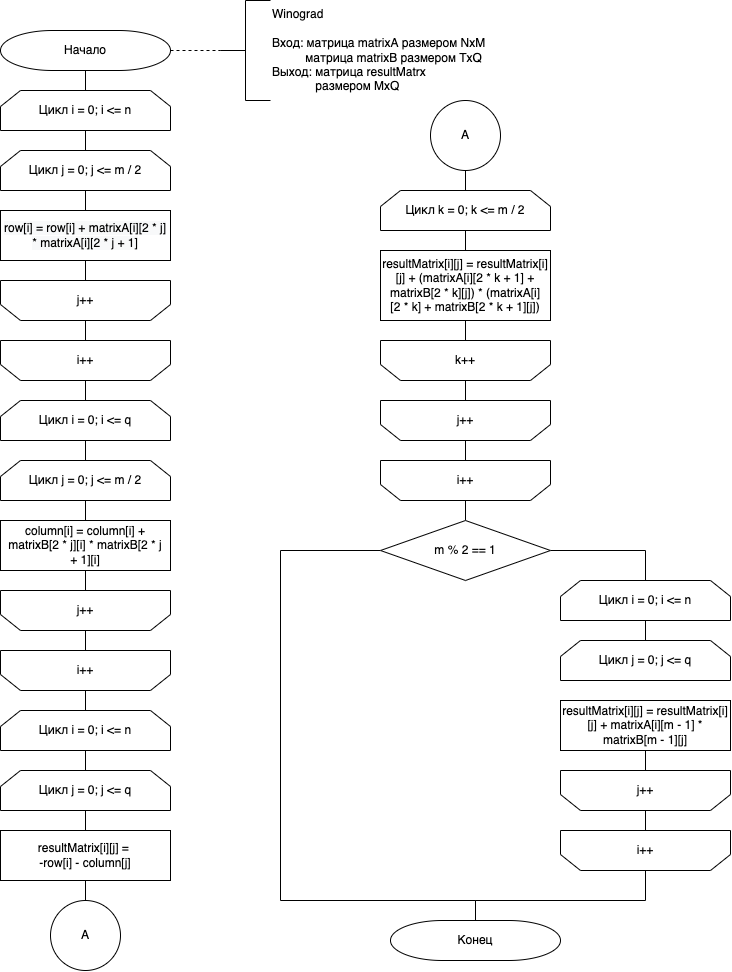
\includegraphics[scale=0.65]{img/Winograd.png}
	\caption{Схема алгоритма Винограда}
	\label{fig:mpr}
\end{figure}

\begin{figure}[ht!]
	\centering
	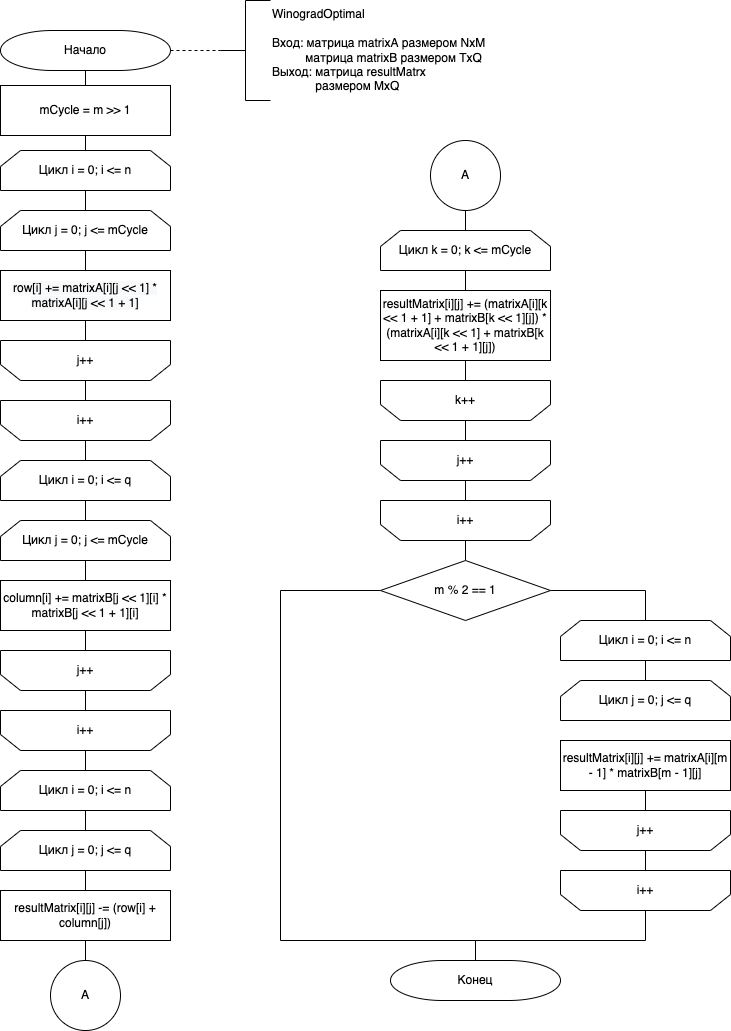
\includegraphics[scale=0.65]{img/WinogradOptimal.png}
	\caption{Схема функций оптимизированного алгоритма Винограда}
	\label{fig:mpr}
\end{figure}

\section{Модель вычислений}

Для последующего вычисления трудоемкости введём модель вычислений.

\begin{enumerate}
	\item Операции из списка (\ref{for:opers}) имеют трудоемкость 1.
	\begin{equation}
	\label{for:opers}
	+, -, /, \%, ==, !=, <, >, <=, >=, [], ++, {-}-
	\end{equation}
	\item Трудоемкость оператора выбора if условие then A else B рассчитывается по формуле (\ref{for:if}).
	\begin{equation}
	\label{for:if}
	f_{if} = f_{\text{условия}} +
	\begin{cases}
	f_A, & \text{если условие выполняется,}\\
	f_B, & \text{иначе.}
	\end{cases}
	\end{equation}
	\item Трудоемкость цикла рассчитывается по формуле (\ref{for:for}).
	\begin{equation}
	\label{for:for}
	f_{for} = f_{\text{инициализации}} + f_{\text{сравнения}} + N(f_{\text{тела}} + f_{\text{инкремента}} + f_{\text{сравнения}})
	\end{equation}
	\item Трудоемкость вызова функции равна 0.
\end{enumerate}

\section{Трудоёмкость алгоритмов}

\subsection{Стандартный алгоритм умножения матриц}

Трудоёмкость стандартного алгоритма умножения матриц можно вычислять поэтапно.
\begin{itemize}
	\item Трудоёмкость внешнего цикла по $i \in [1..A]$ вычисляется как $f = 2 + A \cdot (2 + f_{body})$.
	\item Трудоёмкость цикла по $j \in [1..C]$ вычисляется как $f = 2 + C \cdot (2 + f_{body})$.
	\item Трудоёмкость скалярного умножения двух векторов -- цикл по $k \in [1..B]$ вычисляется как $f = 2 + 10B$.
\end{itemize}

Трудоёмкость стандартного алгоритма равна трудоёмкости внешнего цикла, можно вычислить ее, подставив циклы тела, что выполнено в формуле (\ref{for:base}).
\begin{equation}
	\label{for:base}
	f_{base} = 2 + A \cdot (4 + C \cdot (4 + 10B)) = 2 + 4A + 4AC + 10ABC \approx 10ABC
\end{equation}

\subsection{Алгоритм Винограда}

Трудоёмкость алгоритма Винограда можно вычислять поэтапно.

\begin{enumerate}
	\item Трудоёмкость создания векторов rows и cols вычисляется как (\ref{for:init}).
	\begin{equation}
	\label{for:init}
	f_{create} = A + C.
	\end{equation}
	
	\item Трудоёмкость заполнения вектора rows вычисляется как (\ref{for:MH}).
	\begin{equation}
	\label{for:MH}
	f_{rows} = 3 + \frac{B}{2} \cdot (5 + 12A).
	\end{equation}
	
	\item Трудоёмкость заполнения вектора cols вычисляется как (\ref{for:MV}).
	\begin{equation}
	\label{for:MV}
	f_{cols} = 3 + \frac{B}{2} \cdot (5 + 12C).
	\end{equation}
	
	\item Трудоёмкость цикла заполнения матрицы для чётных размеров вычисляется как (\ref{for:cycle}).
	\begin{equation}
	\label{for:cycle}
	f_{cycle} = 2 + A \cdot (4 + C \cdot (11 + \frac{25}{2} \cdot B)).
	\end{equation}
	
	\item Трудоёмкость цикла, для дополнения умножения суммой последних нечётных строки и столбца, если общий размер нечётный вычисляется как (\ref{for:last}).
	\begin{equation}
	\label{for:last}
	f_{last} = \begin{cases}
	2, & \text{чётная,}\\
	4 + A \cdot (4 + 14C), & \text{иначе.}
	\end{cases}
	\end{equation}
\end{enumerate}

Итого, для худшего случая (нечётный размер матриц): 
\begin{equation}
\label{for:bad}
f_{wino\_w} = A + C + 12 + 8A + 5B + 6AB + 6CB + 25AC + \frac{25}{2}ABC \approx 12.5 \cdot MNK.
\end{equation}

Для лучшего случая (чётный размер матриц): 
\begin{equation}
\label{for:good}
f_{wino\_b} = A + C + 10 + 4A + 5B + 6AB + 6CB + 11AC + \frac{25}{2}ABC \approx 12.5 \cdot MNK.
\end{equation}

\subsection{Оптимизированный алгоритм Винограда}

Трудоёмкость улучшенного алгоритма Винограда можно вычислять поэтапно. 
\begin{enumerate}
	\item Трудоёмкость создания векторов rows и cols высчитывается по формуле (\ref{for:impr_init}).
	\begin{equation}
	\label{for:impr_init}
	f_{init} = A + C.
	\end{equation}
	
	\item Трудоёмкость заполнения вектора rows высчитывается по формуле (\ref{for:impr_MH}).
	\begin{equation}
	\label{for:impr_MH}
	f_{rows} = 2 + \frac{B}{2} \cdot (4 + 8A).
	\end{equation}
	
	\item Трудоёмкость заполнения вектора cols высчитывается по формуле (\ref{for:impr_MV}).
	\begin{equation}
	\label{for:impr_MV}
	f_{cols} = 2 + \frac{B}{2} \cdot (4 + 8A).
	\end{equation}
	
	\item Трудоёмкость цикла заполнения матрицы для чётных размеров высчитывается по формуле (\ref{for:impr_cycle}).
	\begin{equation}
	\label{for:impr_cycle}
	f_{cycle} = 2 + A \cdot (4 + C \cdot (8 + 9B)).
	\end{equation}
	
	\item Трудоёмкость цикла, для дополнения умножения суммой последних нечётных строки и столбца, если общий размер нечётный высчитывается по формуле (\ref{for:impr_last}).
	\begin{equation}
	\label{for:impr_last}
	f_{last} = 
	\begin{cases}
	2, & \text{чётная,}\\
	4 + A \cdot (4 + 12C), & \text{иначе.}
	\end{cases}
	\end{equation}
\end{enumerate}

Итого, для худшего случая (нечётный общий размер матриц) имеем формулу (\ref{for:bad_impr}).
\begin{equation}
\label{for:bad_impr}
f = A + C + 10 + 4B + 4BC + 4BA + 8A + 20AC + 9ABC \approx 9ABC.
\end{equation}

Для лучшего случая (чётный общий размер матриц) имеем формулу (\ref{for:good_impr}).
\begin{equation}
\label{for:good_impr}
f = A + C + 8 + 4B +4BC + 4BA + 4A + 8AC + 9ABC \approx 9ABC.
\end{equation}

\section{Вывод}
На основе теоретических данных, полученных из аналитического раздела, были построены схемы обоих алгоритмов умножения матриц.  Оценены их трудоёмкости в лучшем и худшем случаях.
